\documentclass{article}

\usepackage{amsmath}
\usepackage{listings}
\usepackage{graphicx}


\title{Data Analysis and Visualisation using R}
\date{2016-01-11}
\author{\textbf{Wing Cheung Kenneth Lui} \\
Computer Laboratory, University of Cambridge \\
{\tt wckl2@cam.ac.uk}}

\begin{document}
  \pagenumbering{arabic}
  \maketitle

\section{Introduction}

In this study, we analyse a training dataset provided in CSV (comma-separated values) format. There are 1800 observations (i.e. rows) and 12 columns of values in total. The first column, named {\tt id}, contains unique integer identifiers from 1 to 1800; the second column, named {\tt Y}, stores a number without containing any {\tt NA} values; {\tt Y} is followed by nine floating point numeric columns named from {\tt X1}, {\tt X2},  \(...\), {\tt X9}, which may contain {\tt NA}s in some observations; finally, the last column, named {\tt label}, contains one of eight text values such as ash, beech, oak and so on.

We divide the data into eight uneven subsets based on the label value. During preprocessing, {\tt id}, {\tt label} and {\tt NA} entries are removed from each subset. The number of observations and the remaining column names is tabulated in Table~\ref{subset-table}. In statistical learning context, the training data are observations where the response variable Y may have some relationship with one or more of the potential predictor variables {\tt X\textsubscript{i}}.

\begin{table}
\begin{center}
\begin{tabular}{|c|c|c|}
\hline \bf Label & \bf Number of observations & \bf Predictor variables \\ \hline
ash & 500 & {\tt X1, X2, X3, X4, X5, X6, X7, X8, X9} \\ \hline
beech & 500 & {\tt X3, X7} \\ \hline
elder & 500 & {\tt X7} \\ \hline
elm & 100 & {\tt X3, X8} \\ \hline
larch & 50 & {\tt X3, X4, X5, X9} \\ \hline
oak & 50 & {\tt X3} \\ \hline
rowan & 50 & {\tt X4} \\ \hline
yew & 50 & {\tt X4} \\ \hline
\end{tabular}
\end{center}
\caption{\label{subset-table} Overview of subset in training data.}
\end{table}

\section{Statistical Analyses}

A variety of regression and classification techniques have been employed to detect characteristics and dependencies underlying the training data. The results are presented graphically and numerically in this report.

\begin{table}
\begin{center}
\begin{tabular}{|c|c|}
\hline \bf Library & \bf Functions provided \\ \hline
{\textit class} & {\tt knn(), cv.knn()} \\ \hline
{\textit glmnet} & {\tt cv.glmnet()} \\ \hline
{\textit leaps} & {\tt regsubsets()} \\ \hline
{\textit MASS} & {\tt lda(), qda()} \\ \hline
\end{tabular}
\end{center}
\caption{\label{library-table} Overview of libraries used.}
\end{table}

\subsection{Ash subset}

The response variable {\tt Y} is continuous so regression methods are used. First, we use {\tt pairs()} to produce a matrix of pairwise scatterplots for each pair of variables ({\tt Y} and all {\tt X\textsubscript{i}}) to detect whether any observable patterns exist. {\tt X7} shows an obvious linear relationship with {\tt Y} in these plots so we use {\tt lm()} to fit a \textbf{simple linear regression} between them. The summary of this fit shows that the least squares coefficients of {\tt X7} in the linear relationship are highly significant (p-value is close to zero). Its training $R^2$ value of 0.9966 shows that the variance left unexplained by the linear fit is negligible. This fit also results in a convincing inspection plot as shown in Figure~\ref{fig:01-ash}. No obvious pattern can be seen in the residuals vs fitted values plot. However, this should not rule out the possibility that {\tt Y} is also related to some other predictors. we perform a \textbf{multiple linear regression} using all available predictors and obtain an ``improved'' fit where both {\tt X3} and {\tt X7} are significant and training $R^2$ value is 0.9988. But such improvement must be taken with a grain of salt because {\em training $R^2$ values for any more flexible models (i.e. those with more predictors) must be no less than a more restrictive one}. To verify whether a simple linear model involving {\tt X7} only is the true relationship over other more flexible multiple linear models, 5-fold cross-validation has been used with best subset variables selection. As shown in Listing~\ref{ash}, cross-validation suggests $Y \sim X3+X4+X7+X8$ as the model achieving the lowest test squared error but the performance difference compared to $Y \sim X3$ is small, which is chosen for the sake of interpretability.

\begin{figure}[h!]
  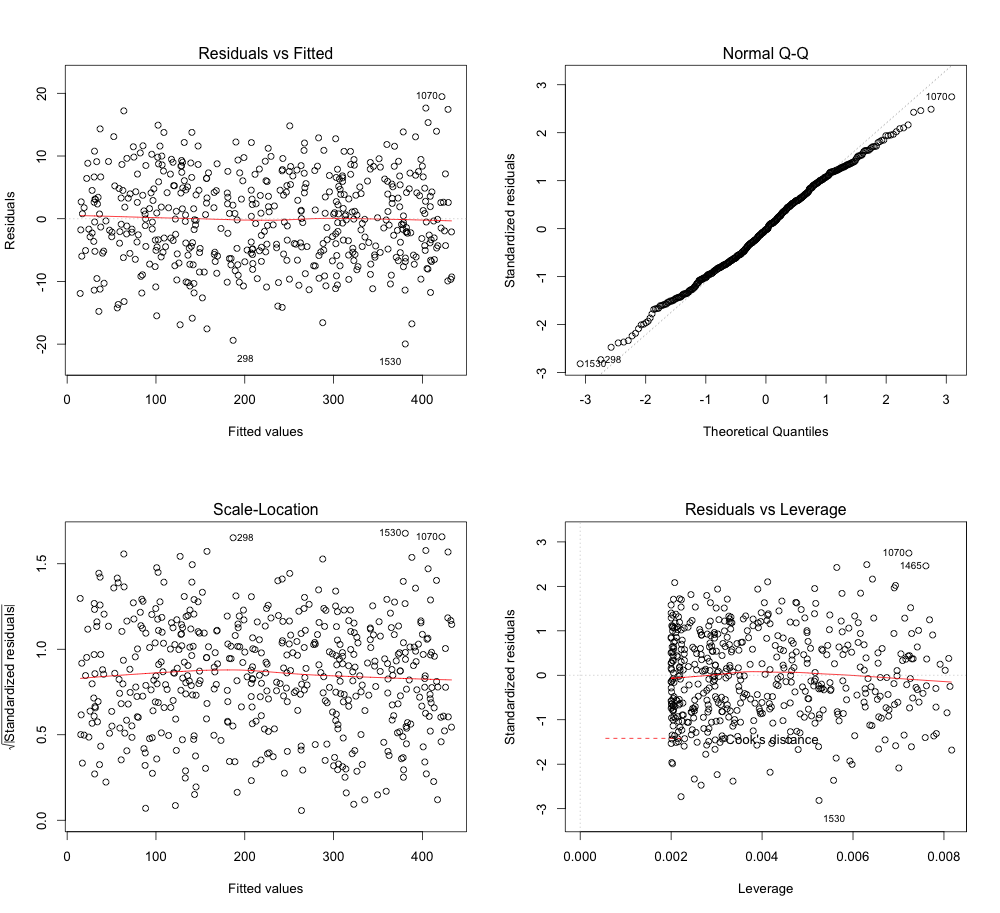
\includegraphics[width=\linewidth]{project/images/01-ash.png}
  \caption{Inspection plots for linear fit $Y \sim X7$ in ash dataset.}
  \label{fig:01-ash}
\end{figure}

\subsection{Beech subset}

We approach the problem from a classification perspective because the response variable Y is binary (either 0 or 1). In a binary classification problem, it is helpful to plot all the data points on the same scatter plot using distinct symbols to visualise how the two classes are separated, as shown in Figure~\ref{fig:02-beech}. While the separation between the two classes is not absolutely clear, the boundary seems to be linear rather than quadratic. We first randomly divide the data into a training set and a test set so we can quantitatively compare models given by  \textbf{logistic regression},  \textbf{linear discriminant analysis (LDA)} and  \textbf{quadratic discriminant analysis (QDA)}. These three methods achieve test classification accuracies at 89.6\%, 90.8\% and 89.6\% respectively. This result suggests that the class boundary is linear, so the flexibility ``gained'' by using QDA is not useful to offset the extra errors caused by {\em variability} in the model. While both logistic regression and LDA model a linear boundary, LDA's slight performance gain over logistic regression may be explained by LDA's assumption. Its assumption states that predictors are drawn from a multivariate Gaussian distribution with a class-specific mean vector and a common covariance matrix. By inspecting the mean vector and covariance matrix computed for each class, LDA's assumption appears to be correct on this training data set. We also experiment with \textbf{k-Nearest Neighbors (KNN)} classification but it does not give significantly different results.

\begin{figure}[h!]
  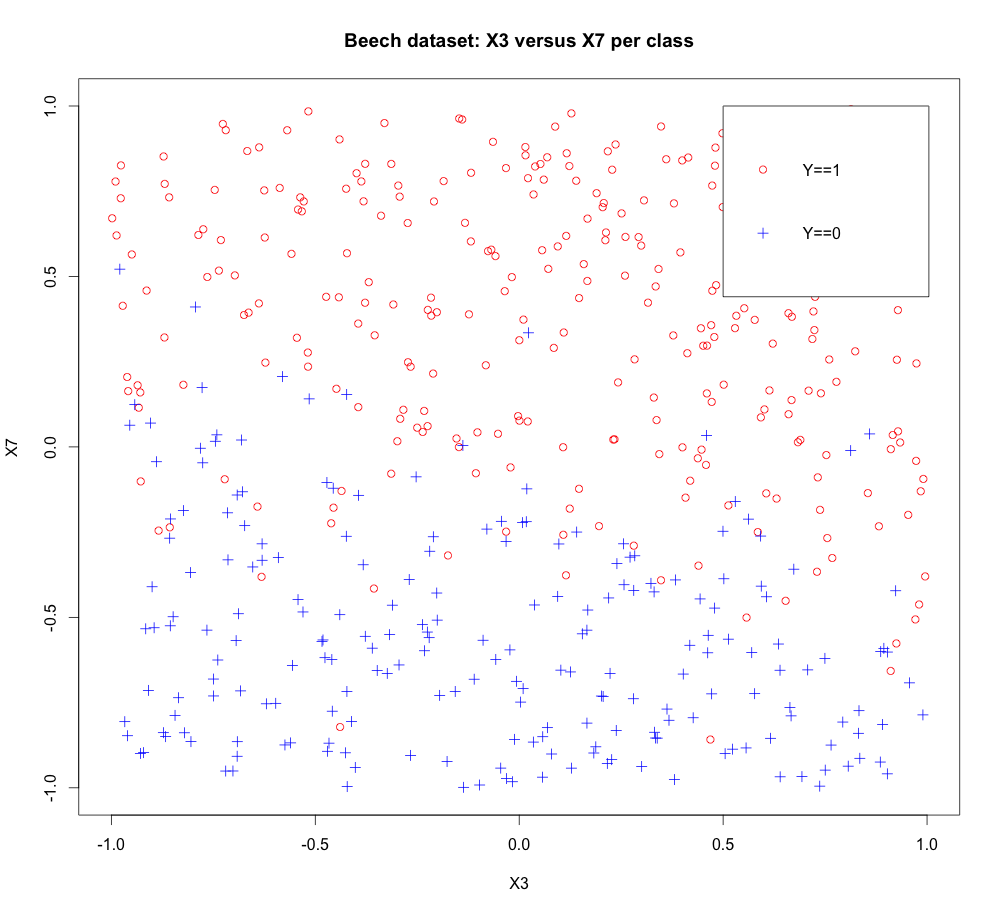
\includegraphics[width=\linewidth]{project/images/02-beech.png}
  \caption{Inspection plot for decision boundary in beech dataset.}
  \label{fig:01-beech}
\end{figure}

\subsection{Elder subset}

We start exploring this set of data by plotting a scatterplot between {\tt Y} and {\tt X7}, the only remaining predictor. We observe that a funnel shape formed by the data points overshadows an upward linear relationship, as shown in Figure~\ref{fig:03-elder}. The funnel shape may imply a non-constant variance in the error terms, a phenomenon called {\em heteroscedasticity}. In this data set, heteroscedasticity causes the variance in error terms increases with the response values. One possible solution is transforming the response variable using a concave function hence we compare three models: $Y \sim X7$, $log(Y) \sim X7$ and $\sqrt{Y} \sim X7$. The funnel-shaped pattern and magnitude observed in the residuals versus fitted values plot for the simple linear regression model has been greatly reduced in Figure~\ref{fig:04-elder}, although not completely eliminated, through the use of concave transformation. The training $R^2$ values for these models are 0.3359, 0.3305 and 0.3373 respectively. Based on this, we have chosen $sqrt{Y} \sim X7$ as the resulting linear regression coefficients are significant.

\begin{figure}[h!]
  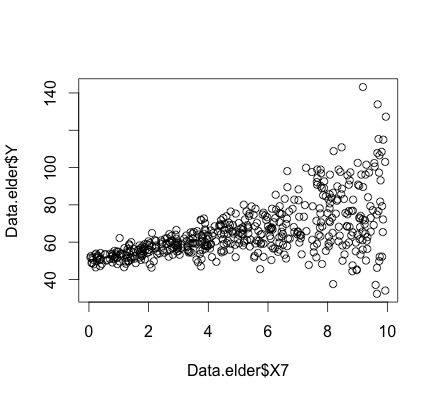
\includegraphics[width=\linewidth]{project/images/03-elder.png}
  \caption{Inspection plot for heteroscedasticity in elder dataset.}
  \label{fig:03-elder}
\end{figure}

\begin{figure}[h!]
  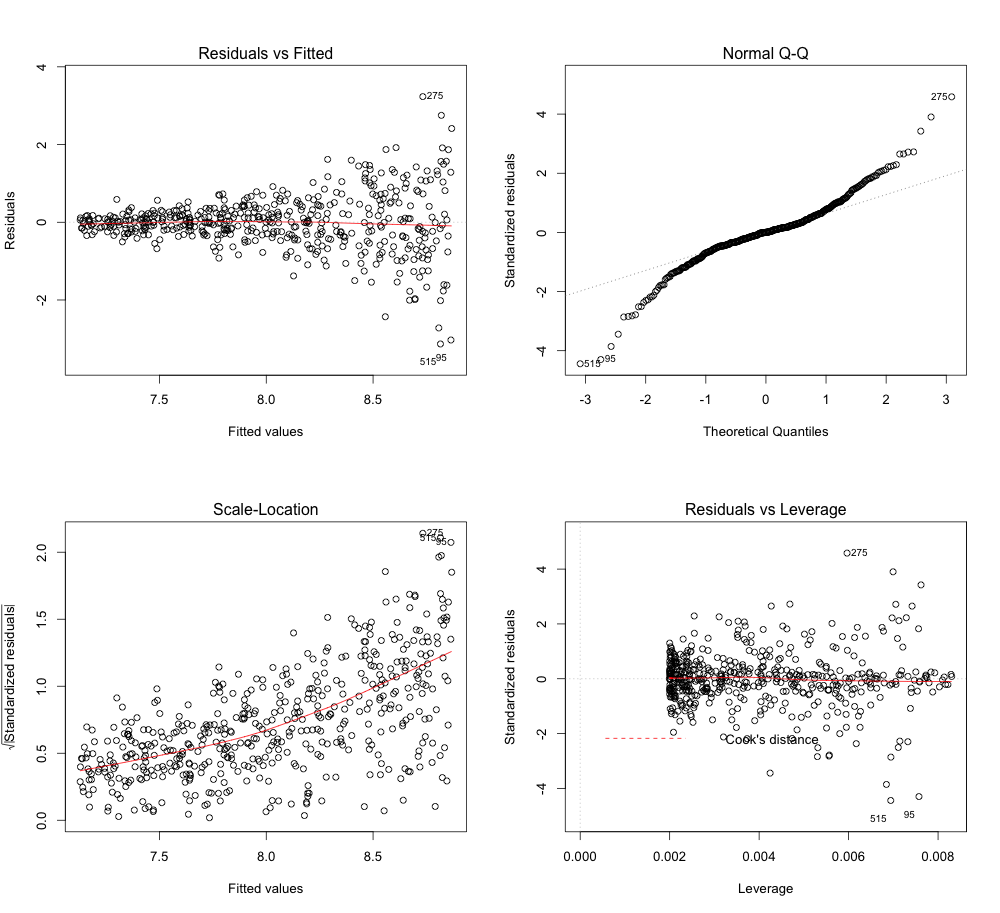
\includegraphics[width=\linewidth]{project/images/04-elder.png}
  \caption{Inspection plots showing reduced funnel-shape residuals for $\sqrt{Y} \sim X7$ in elder dataset.}
  \label{fig:04-elder}
\end{figure}

\subsection{Elm subset}

Since the response variable Y is qualitative (represented in 0 or 1), we perform classification analysis similar to the beech subset. A difference noticeable by inspecting the scatter plot (Figure~\ref{fig:05-elm}) is that the two classes are more well-separated in this data set compared to the beech subset. We follow the same approach, divide the data into a training set and a test set, then apply logistic regression, LDA and QDA to the training set. Surprisingly, these three methods give the exact same prediction for the test set and their prediction accuracy is 90.2\% on the test set. On the other hand, it may be interesting to compare these three parametric methods with a non-parametric method, namely k-nearest neighbour (KNN). Before applying KNN, the predictors should be {\em standardized} to have zero mean and unit variance. we perform three KNN predictions on the standardized data with {\tt K}=1, 3 and 10. A larger K, which specifies the number of nearest neighbour to be considered, implies less variance in the model and higher bias. Despite this conceptual bias-variance trade-off, we achieve exactly the same 87.8\% prediction accuracy rate on the test set regardless of our choice of {\tt K}. The predictions given by {\tt K}=1 and {\tt K}=3 are exactly the same and they are different from {\tt K}=10 by two predictions. we think the parametric methods outperform the non-parametric KNN method because the underlying classification boundary is linear so a simpler model is less prone to noise in the data. The flexibility of KNN method is an overkill and does not cause a comparative advantage.

\begin{figure}[h!]
  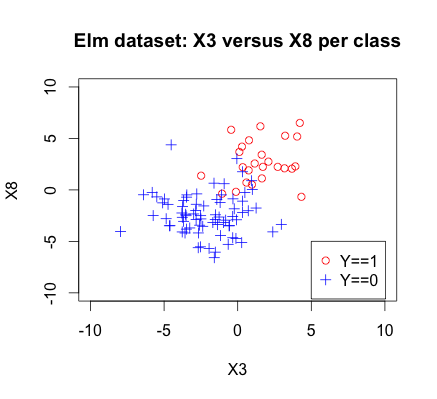
\includegraphics[width=\linewidth]{project/images/05-elm.png}
  \caption{Inspection plot for decision boundary in elm dataset.}
  \label{fig:05-elm}
\end{figure}

\subsection{Larch subset}

Among predictor columns {\tt X3, X4, X5} and {\tt X9}, we observe an evident linear relationship between {\tt Y} and {\tt X5} in the pairwise scatterplots (Figure~\ref{fig:06-larch}) for every pair of variables ({\tt Y} and the predictors). A hypothesis we have about this data set is that some of the predictors are irrelevant to the response variable Y, so I decide to apply \textbf{variable selection techniques} using {\tt regsubsets()} with the \textbf{best subset}, \textbf{forward stepwise} and \textbf{backward stepwise approach}. The three approaches gave exactly the same set of predictors for each number of predictors. As this data set is smaller than the previous subsets, we use 5-fold cross-validation instead of validation set approach to choose among the models. Finally, the model using all predictors (i.e. $Y \sim X3+X4+X5+X9$) achieve the lowest 5-fold cross-validated test error. The result is confirmed by a multiple linear regression fit using all these predictors where every predictor is associated with a low p-value and the training $R^2$ is as high as 0.9593. No outliers or high leverage points can be observed from the four default plots (Figure~\ref{fig:07-larch}) for the linear model.

\begin{figure}[h!]
  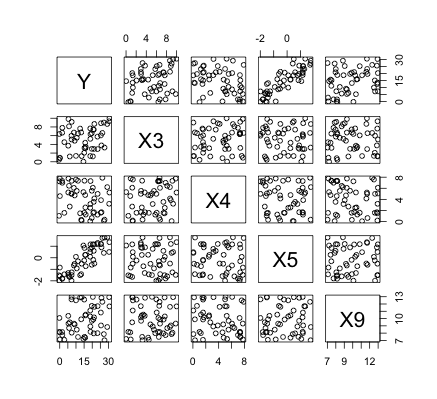
\includegraphics[width=\linewidth]{project/images/06-larch.png}
  \caption{Inspection plot for pairwise correlation in larch dataset.}
  \label{fig:06-larch}
\end{figure}

\begin{figure}[h!]
  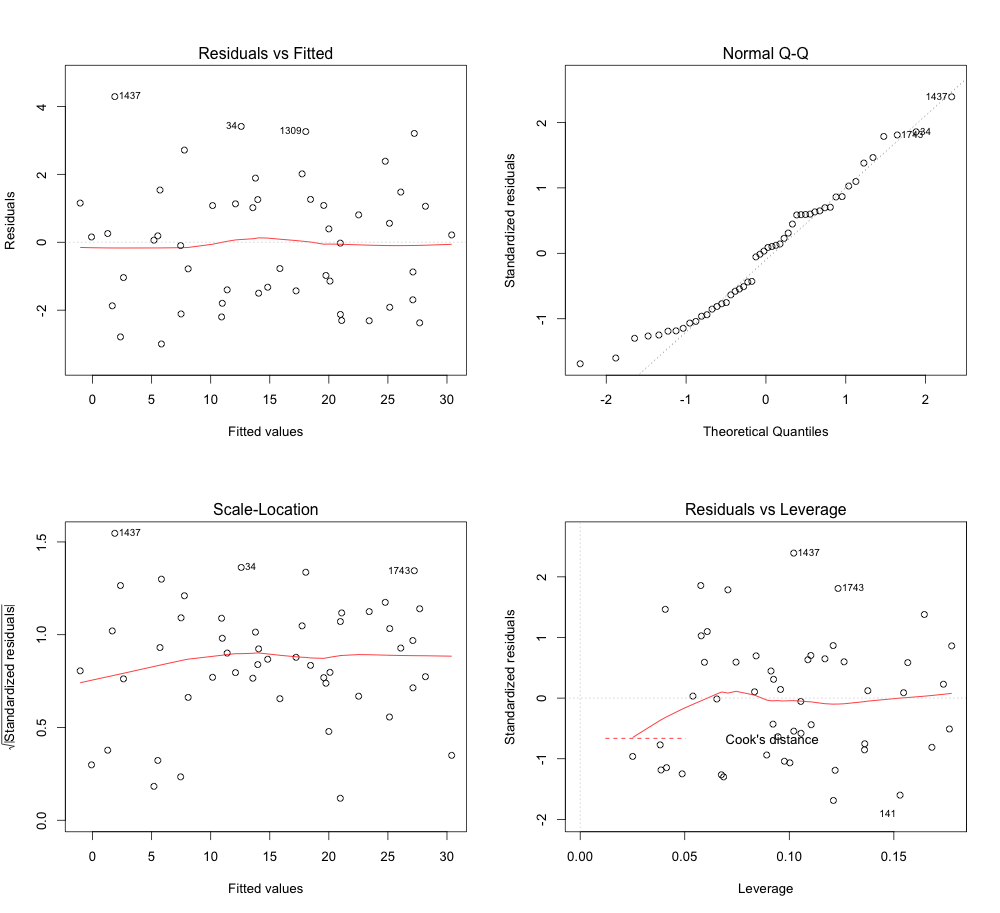
\includegraphics[width=\linewidth]{project/images/07-larch.png}
  \caption{Inspection plots showing good linear fit for $\sqrt{Y} \sim X3+X4+X5+X9$ in larch dataset.}
  \label{fig:07-larch}
\end{figure}

\subsection{Oak subset}

An inspection using scatter plot (Figure~\ref{fig:08-oak}) identifies a nonlinear relationship between $Y$ and the only predictor, namely $X3$. Plotting Y against increasing powers of $X3$ shows that $Y$ seems to have linear relationship with $X3^4$ or $X3^5$. Hence, we use {\tt poly()} function to produce a matrix with polynomial values for $X3$ up to $X3^8$, then perform best subset model selection with {\tt regsubsets()} and then apply 5-fold cross-validation to choose from these candidate models which have different number of predictors. The lowest cross-validated test error is obtained by using three terms in the model. We perform the best subset model selection again (using all data instead of cross-validation) and pick the model with three terms which are $X3$, $X3^2$ and $X3^4$. The change RSS, adjusted $R^2$, C\textsubscript{p} and BIC versus number of variables is shown in Figure~\ref{fig:09-oak}. in Finally, we fit the data with $Y \sim X3+X3^2+X3^4$ using {\tt lm()} and obtain a training $R^2$ value of 0.975. However, the p-values associated with $X3$ and $X3^2$ terms are not significant. This seems to contradict the result of the ``best model'' using cross-validation. We think that this is caused by {\em collinearity} between the power terms as the different powers of $X3$ are obviously related to each other. Collinearity reduces the accuracy of the regression coefficient estimation as well as the probability of correctly detecting a non-zero coefficient. This hypothesis is supported by the fact that standard errors associated with the coefficients in the ``three terms model'' is 10 times larger than the standard errors in the condition when only one power-term is used as predictors. As 5-fold cross-validated test error is a direct estimate for the true test error, we are confident that it is a more robust way to judge a model's correctness than checking coefficients' p-values (which computation requires estimate of variance from the data). Hence we insist that $Y \sim X3+X3^2+X3^4$ is a good model for the underlying relationship.

\begin{figure}[h!]
  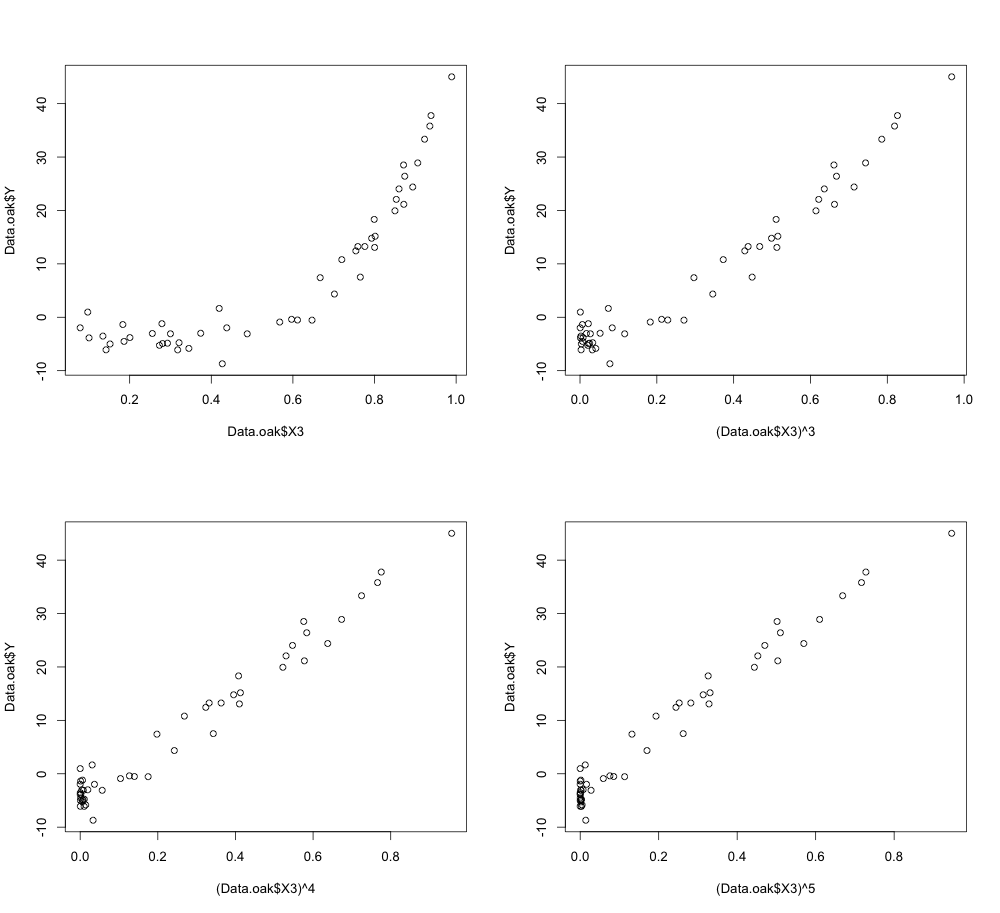
\includegraphics[width=\linewidth]{project/images/08-oak.png}
  \caption{Inspection plot for non-linearity in oak dataset.}
  \label{fig:08-oak}
\end{figure}

\begin{figure}[h!]
  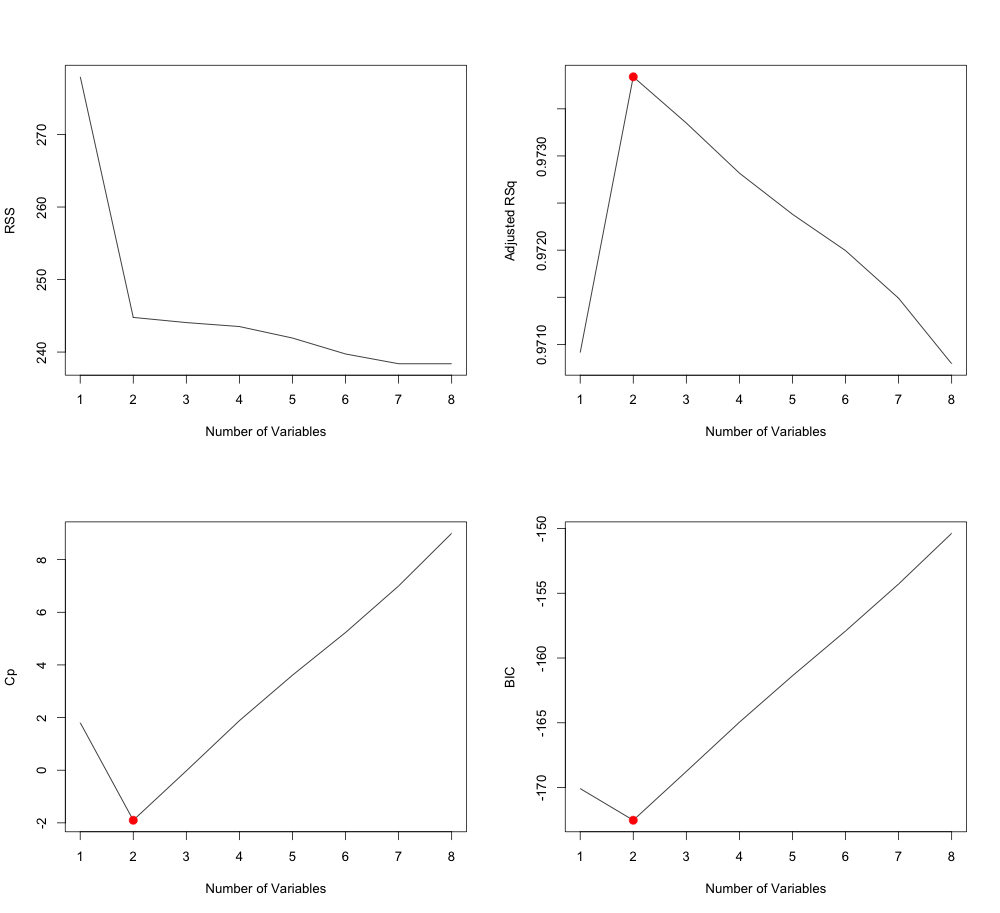
\includegraphics[width=\linewidth]{project/images/09-oak.png}
  \caption{Inspection plots using trend of accuracy versus number of model predictors in oak dataset. The red dots denote minima/maxima.}
  \label{fig:09-oak}
\end{figure}

\subsection{Rowan subset}

The summary of the data shows that the values of $Y$ and $X4$ are evenly spread across their respective ranges. A basic scatterplot (Figure~\ref{fig:10-rowan}) of $X4$ versus $Y$ confirms visually that these observations do not contain any outliers or high leverage points and there is a linear relationship between the response variable $Y$ and the predictor $X4$; the relationship is also supported quantitatively by a close-to-one Pearson correlation coefficient (0.9742865). Hence, we verify the linear relationship by fitting the data using simple linear regression. The best fit line is shown as the red line in Figure~\ref{fig:10-rowan}.The summary of the fitted model shows that the coefficient of $X4$ is statistically significant with an almost-zero p-value. The positive coefficient of $X4$ aligns with the sign of correlation coefficient, which is also positive. The $R^2$ value for the training data is 0.9492 which implies most of the variation in the observation can be explained by the fitted model. There is no apparent pattern in the plot for residuals against fitted values so we can be confident about our hypothesis of a linear relationship. Out of curiosity, I fitted a polynomial regression model with predictors from $X4$, $X4^2$, \(...\) , $X4^5$ and none of the polynomial terms higher than the first power can be fitted to a coefficient significantly.

\begin{figure}[h!]
  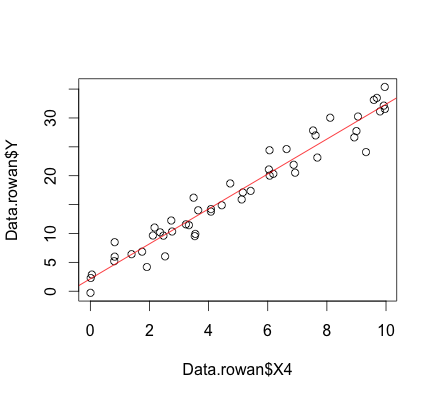
\includegraphics[width=\linewidth]{project/images/10-rowan.png}
  \caption{Inspection plot showing good linear fit for $\sqrt{Y} \sim X3+X4+X5+X9$ in rowan dataset. Best fit line is in red color.}
  \label{fig:10-rowan}
\end{figure}

\subsection{Yew subset}

A simple scatter plot (Figure~\ref{fig:11-yew}) for $Y$ versus $X4$ shows that there are two {\em outliers} (with exceptionally large $Y$ value) and no {\em high leverage point}. While the rest of $Y$ values stay within the range (-1.461, 32.770), those two points have a value of 999. We use {\tt lm()} to fit two simple linear regression models, one on the original data containing the outliers and another one on a clean data set where two outlier points have been removed. In the ``original'' model, least squares fitting fails to identify a significant relationship (i.e. p-value is large) and the model cannot explain the responses? variance (training $R^2$ = 0.02362). In the ``clean'' model, the algorithm finds a significant coefficient for $X4$ (p-value small than 2e-16) and the training $R^2$ is 0.9474 which is able to explain the linear relationship well. An alternative and quantitative measure for this difference is correlation coefficient. The correlation coefficient between $Y$ and $X4$ is -0.1537 when outliers are included but 0.9733695 when outliers are removed. Two outliers, which is 4\% of the observations, are influential enough to prevent a strong positive correlation being detected. Figure~\ref{fig:12-yew} shows the two best fit line corresponding to the ``original'' model (red line) and ``clean'' model (black line). It is also worth investigating which outlier is more influential. Hence, I fit two more models, each using training data with one outlier removed. As we can see from the plot, one outlier is associated with an extreme $X4$ value but the other one is associated with a $X4$ value closer to the average. Figure~\ref{fig:13-yew} clearly shows the impact of the outliers. The blue line represents the outlier-free best fit line, which aligns well with the data points. The red line represent the best fit line when both outliers are present so this line is furthest away from the blue line. The green line is the best fit line trained on all data except the outlier observation with close-to-mean $X4$ value. The orange line is the best fit line trained on all data except the outlier observation with extreme $X4$ value. The orange line is closer to the blue line than the green one so we can say that it is less influenced by an outlier. In other words, the outlier with extreme $X4$ value has had a larger impact than the one with average $X4$ value on the correctness of the best fit line. This demonstrate the leverage concept - extreme $X$ value has high leverage while average $X$ value has low leverage. Leverage statistics can be computed using {\tt hatvalues()}, the outlier with extreme $X4$ value has a leverage of 0.0721, which is close to the maximum (0.0756), while the one with average $X4$ value has a leverage of 0.0224, which is close to the minimum (0.0202).

\begin{figure}[h!]
  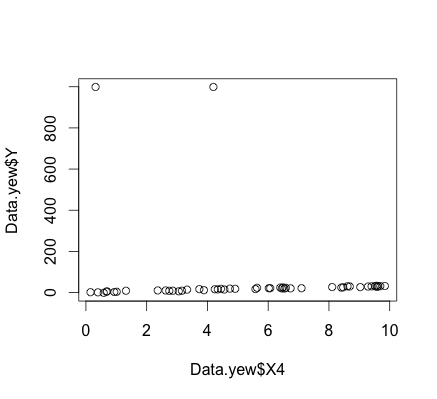
\includegraphics[width=\linewidth]{project/images/11-yew.png}
  \caption{Inspection plot showing outliers in yew dataset.}
  \label{fig:11-yew}
\end{figure}

\begin{figure}[h!]
  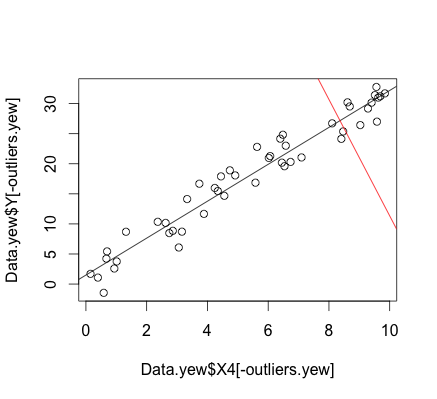
\includegraphics[width=\linewidth]{project/images/12-yew.png}
  \caption{Inspection plot showing impact of outliers on linear fit models in yew dataset.}
  \label{fig:12-yew}
\end{figure}

\begin{figure}[h!]
  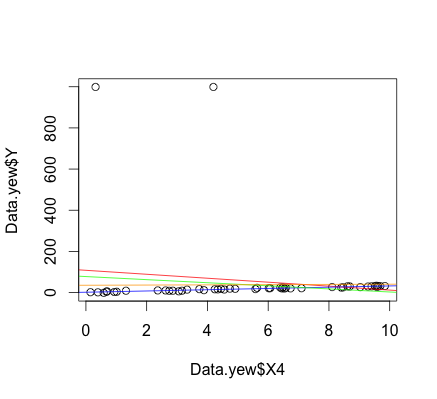
\includegraphics[width=\linewidth]{project/images/13-yew.png}
  \caption{Inspection plot comparing the impact of outliers on linear fit models in yew dataset.}
  \label{fig:13-yew}
\end{figure}

\section{Conclusion}

In this study, we have applied various statistical learning methods. The lesson learnt is that outliers and high leverage points should be identified in the early stage of analysis. Performance of models should be compared using independent test set or cross-validation because any metrics obtained from the training data may be impacted by {\em overfitting}.

\clearpage


\paragraph{Appendices}

\lstinputlisting[breaklines=true,language=R,caption={sharecode.R},label=sharedcode]{project/1-sharedcode.R}

\rule{\textwidth}{1pt}

\lstinputlisting[breaklines=true,language=R,caption={preprocessing.R},label=preprocessing]{project/2-preprocessing.R}

\rule{\textwidth}{1pt}

\newpage

\lstinputlisting[breaklines=true,language=R,caption={ash.R},label=ash]{project/3-ash.R}

\rule{\textwidth}{1pt}

\lstinputlisting[breaklines=true,language=R,caption={beech.R},label=beech]{project/4-beech.R}

\rule{\textwidth}{1pt}

\lstinputlisting[breaklines=true,language=R,caption={elder.R},label=elder]{project/5-elder.R}

\rule{\textwidth}{1pt}

\lstinputlisting[breaklines=true,language=R,caption={elm.R},label=elm]{project/6-elm.R}

\rule{\textwidth}{1pt}

\lstinputlisting[breaklines=true,language=R,caption={larch.R},label=larch]{project/7-larch.R}

\rule{\textwidth}{1pt}

\lstinputlisting[breaklines=true,language=R,caption={oak.R},label=oak]{project/8-oak.R}

\rule{\textwidth}{1pt}

\lstinputlisting[breaklines=true,language=R,caption={rowan.R},label=rowan]{project/9-rowan.R}

\rule{\textwidth}{1pt}

\lstinputlisting[breaklines=true,language=R,caption={yew.R},label=yew]{project/10-yew.R}

\rule{\textwidth}{1pt}

\end{document}